\documentclass[UTF8]{ctexart}							   
%导言区
\usepackage{authblk}
\usepackage{cite}
\usepackage{graphicx}
\usepackage{subfigure}
\usepackage{float}
\usepackage{bm}
%使用特殊字体
\usepackage{fontspec}
\setmainfont{DejaVu Serif}

\title{超材料研究及其应用浅说}
\author[]{郑卜凡\ 学号:2021302022016}
\affil[]{武汉大学物理科学与技术学院}
\date{\today}
\begin{document}
\maketitle
\begin{abstract}
超材料具有许多自然材料所不具有的奇妙性质,也是如今世界科技的热门前沿领域,属于物理、化学、生物等学科的交叉领域。今年来,关于超材料的研究成果越来越多,
其应用范围也越来越广,本文从超材料的诞生出发,简要的概述了几种热门的超材料类型,并阐述了它们在应用方面的前景和科研方面的进展,涉及少量的原理部分。


\textbf{关键词}:超材料,左手材料,负折射率,电磁场
\end{abstract}

\section{超材料的历史}
\subsection{超材料的概念}
超材料(metamaterial),英文词汇起源于希腊字母μετάmeta,有超出(beyond)的意思。超材料的历史起源于二战后不久发展的微博工程中的人造电解质,
超材料指的是一类具有特殊性质的人工材料,这些材料的性质是自然界中的材料所没有的。比如它们可以让光改变它们的通常性质,这种效果是传统材料无法实现的。它们在成份上
没有什么特别之处,它们的奇特性质源于\textbf{其精密的几何结构以及尺寸大小}\cite{wiki1}。超材料的设计思路富有创造力,这一思想的基础是通过在多种物理结构上的设计来突破某些表观自然规律的限制,从而获得超常的材料功能。超材料的思想昭示人们可以在不违背
基本物理学规律的前提下,人工获得与自然界中的物质具有迥然不同的超常物理性质的“新物质”,把功能材料的设计和开发带入一个崭新的天地。
\subsection{超材料的分类}
目前人类已经探索出来的超材料大致可以分为以下几类:\textit{仿生超材料、生物超材料、智能超材料、软性材料、记忆材料、数字超材料、纳米复合材料、高效防冰材料、自我修复材料、
热电材料、辐射制冷超材料、隔音超材料、声电复合超材料、磁光效应材料、左手材料、光子晶体、量子点、电磁晶体、负曲率光纤、超磁性材料、金属水、离子液体、液态金属、
无声金属、磁性液体、钙钛矿、光操纵材料、电磁隐身超材料、零折射率超材料、负折射率材料、声学超材料、力学结构超材料、弹性超材料、无耗能电子材料、人造介质材料、
频率选择表面、人工磁导体、非正定介质材料、负热膨胀超材料、可重构超表面、复合超表面、时变超表面、双曲超材料、梯度超材料、超疏水材料、莫尔手性超材料、活化太赫兹
超材料、隐身材料(红外隐身材料、雷达隐身材料、可见光隐身材料、声隐身材料、激光隐身材料)、柔性雷达吸波超材料、自修复防腐材料、基于传输线结构的超材料、等离子结
构的超材料、双负(负等效质量密度、负等效弹性模量)弹性超材料}等等\cite{wiki1}
\subsection{早期超材料}
人类对于超材料的研究最先是从负折射率超材料开始的。1968年,前苏联理论物理学家Veselago在理论上预言了,可以通过将介电常数ε和磁导率μ的值全部变为负数产生折射率为负数
的材料,称之为\textbf{左手材料}\cite{RN7}。后来在上个世纪九十年代,理论物理学家J.B.Pendry,从理论上设计了一种结构,可以在整体表现出负折射率\cite{RN19}\cite{RN21}\cite{RN22},后来又连续发表文章
给出了负折射率材料可能的应用,其中就包含“完美透镜”\cite{lens},后来在2001年,研究人员在实验上证实了Pendry的设想(下图一),将理论实践化\cite{RN24}。现在,超材料的生产技术更加成熟,在超材料的基本
设想上,人类又设计出了“气凝胶”\cite{RN12},“自愈性材料\cite{wiki2}”,“辐射制冷材料”,“声学超材料\cite{RN2}”,还有最近几年理论化的导电率100\%的超材料——Stanene\cite{RN9}\cite{wiki3},以及今年(2021年)刚刚表示已经生产成功
的“金属水”\cite{RN13}。人类在改造大自然上已经迈出了一大步,或许在不远的将来,人工制造光学超材料可以使得小说中哈利波特的隐身斗篷成为现实,实现光学隐身。

\begin{figure}[htbp]
\begin{minipage}[t]{0.5\linewidth}
\centering
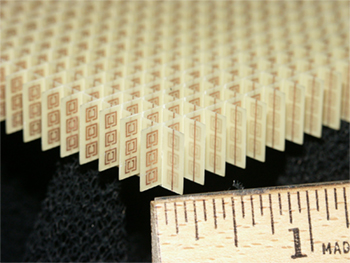
\includegraphics[width=3cm]{fig1.jpg}
\caption{开口谐振环阵列}
\label{fig-1}    
\end{minipage}
\hspace{1ex}
\begin{minipage}[t]{0.5\linewidth}
\centering
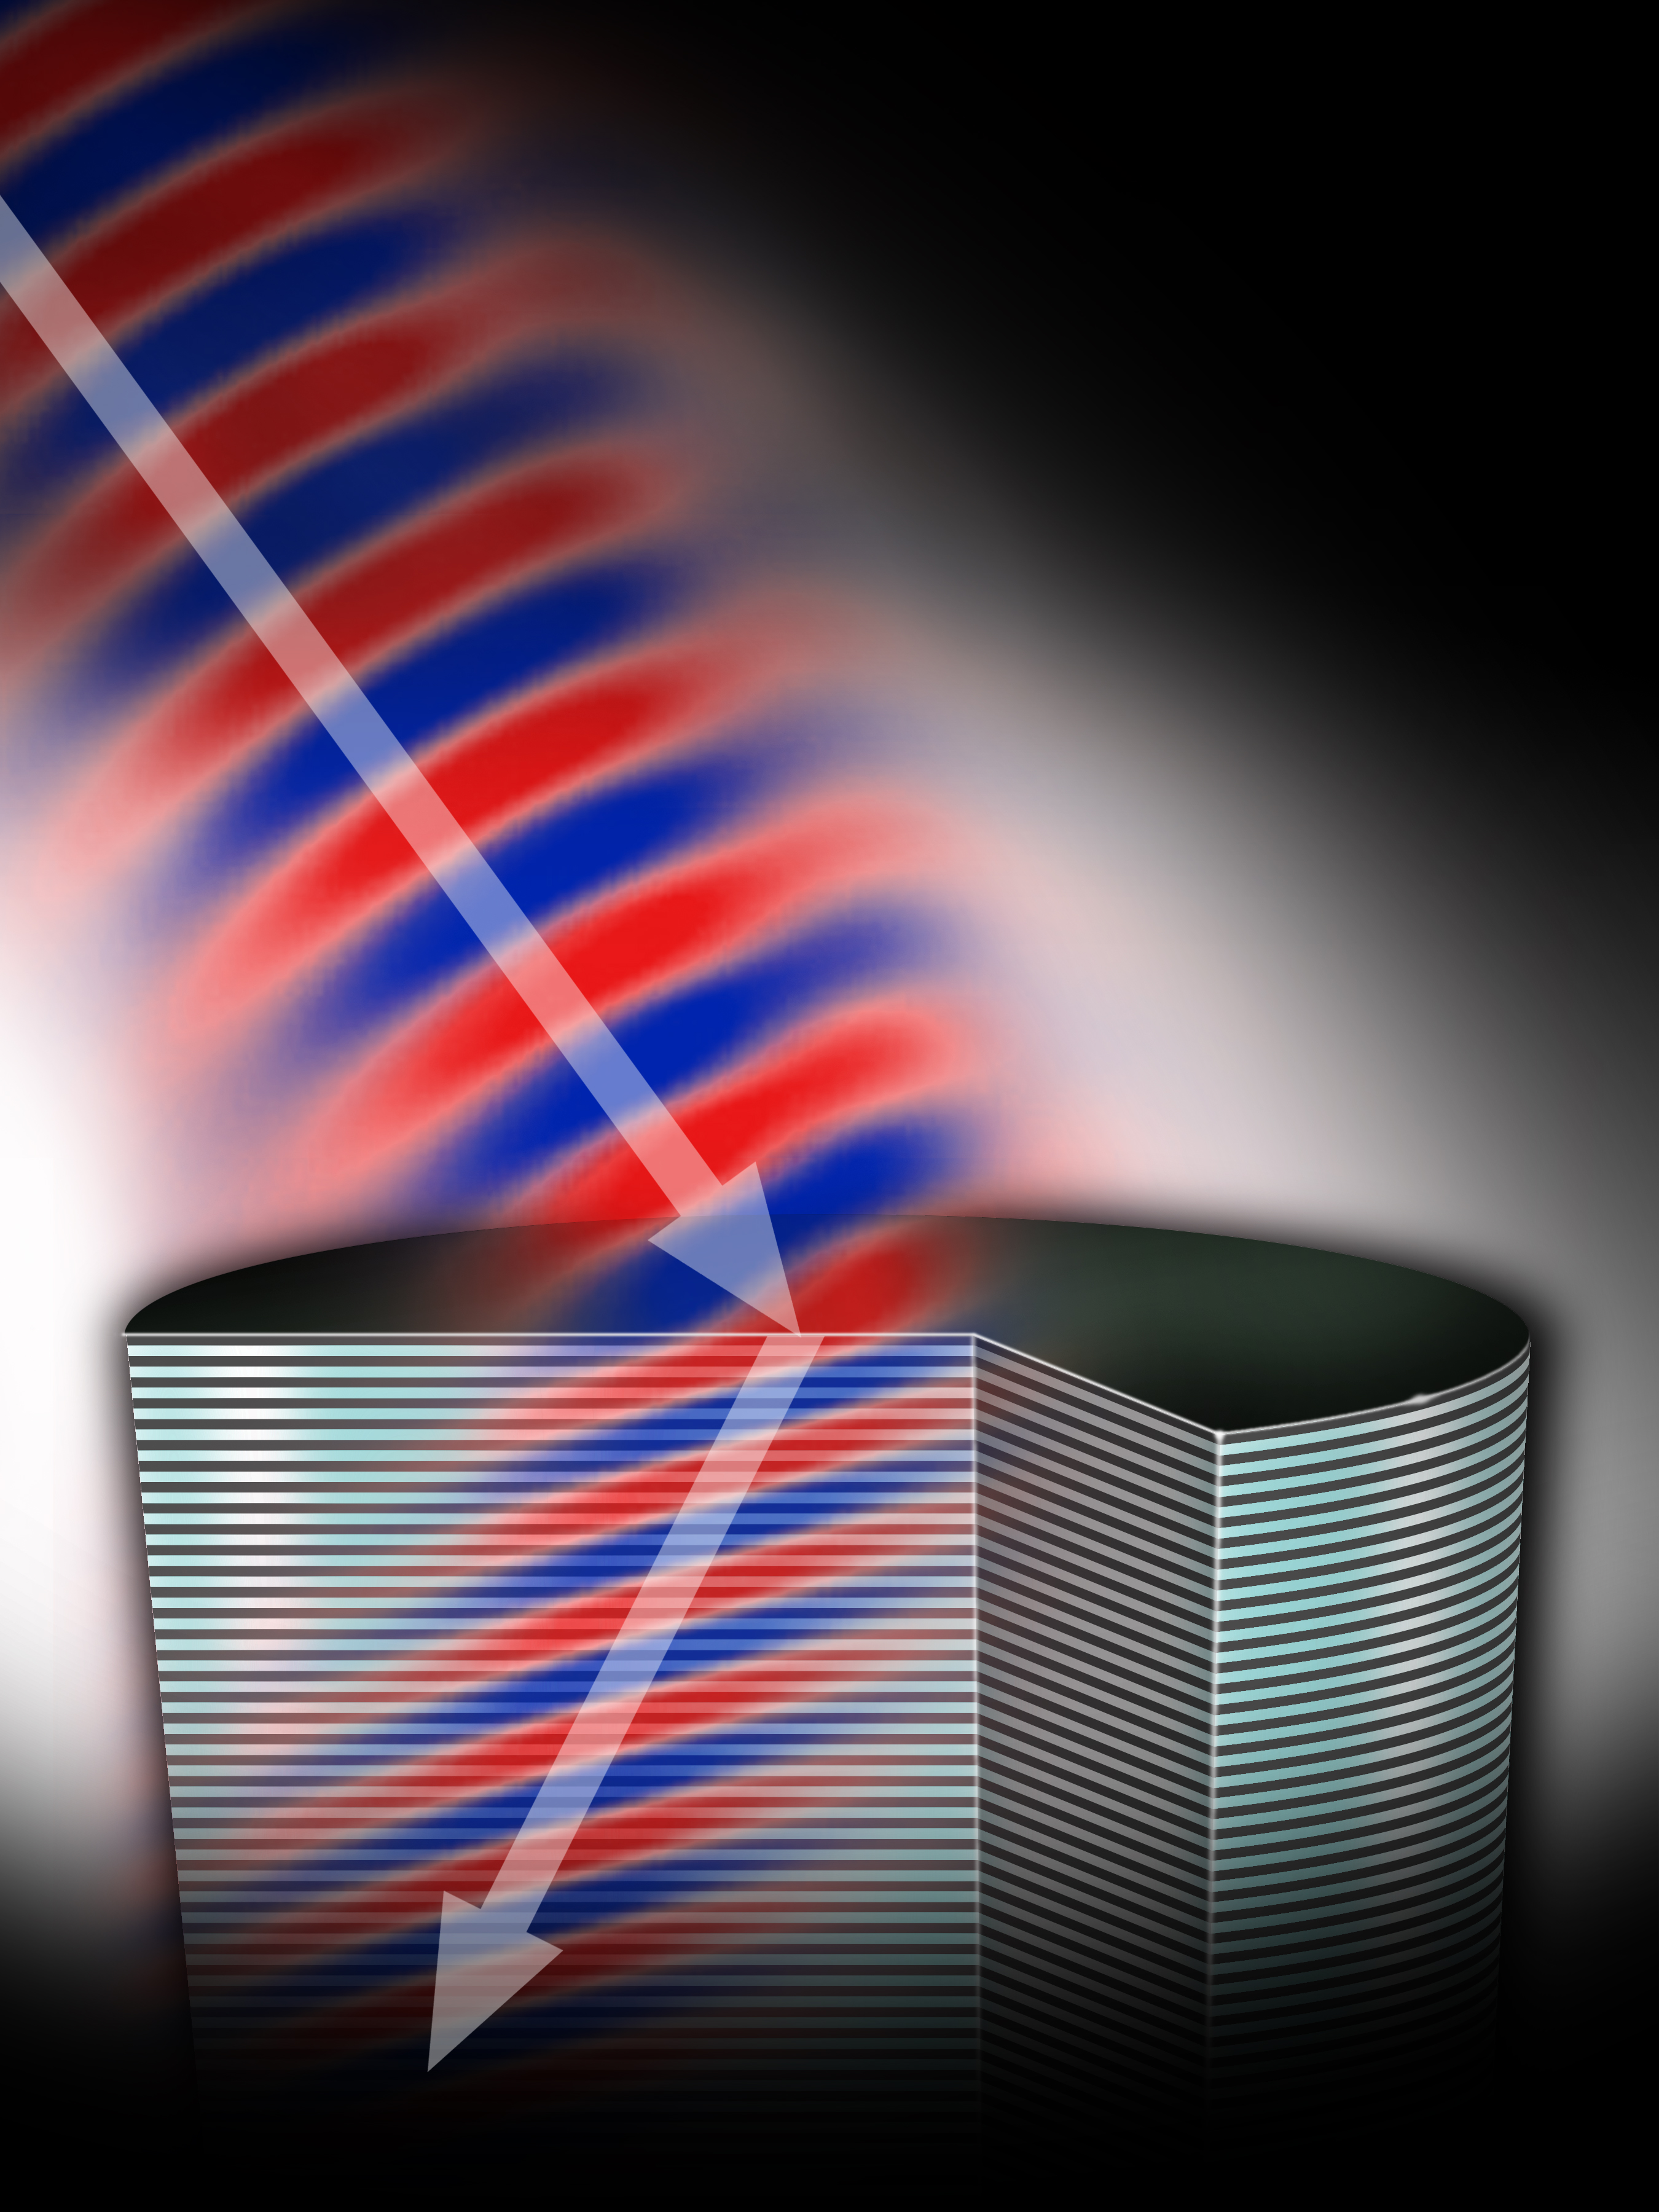
\includegraphics[width=3cm]{fig2.jpg}
\caption{负折射材料中的光的偏折现像}
\label{fig-2}    
\end{minipage}
\end{figure}

\section{电磁超材料简介}
\subsection{电磁超材料的基本原理}
谈到电磁超材料,首先就应该去谈论\textbf{负折射率材料(NIM)},这也是最早出现的关于超材料的设想,本文着重探讨这种材料。


光在普通的介质中传播时,在介质间的分界面会产生折射现象折射角与入射角满足$n_{1}\sin \theta_{1} = n_{2}\sin \theta_{2}$
且入射光线和反射光线分布在法线的异侧,而对于负折射材料而言,光与介质作用后,\textbf{折射光线和反射光线位于法线的同侧}
通常的介质中,波的相速度和群速度是同向的,而在这种负折射材料中相速度和群速度反向。电磁波本身在向外传播时,它的速度依然是光速
,通常意义上所说的波在介质中传播时速度变慢是指\textit{有效速度}变慢了,从电磁波透过介质的原理来看,是由于电磁波会在介质中激起
新的电磁波,新的电磁波与原先的电磁波矢量和构成了真正的电磁波,这个电磁波在振幅和相位方面都会有所变化,折射率就是在宏观上表现
这个表观变化的量,或者可以看作光子在与介质内部粒子碰撞后,走的路径是一种折线,远远大于在真空中的距离,从而导致表观速度变慢。
在费恩曼物理学讲义中feyman给出了下面几个等式\cite{feyman}:
$$
n=1+\frac{q_{e}^{2}}{2\varepsilon_{0}m}\sum_{k}^{} \frac{N_{k}}{\omega _{k}^{2}-\omega ^{2}+i\gamma _{k}\omega } 
$$
$$
n=n^{'}-in^{''}
$$
$$
E_{after\ plate}=e^{-\omega n^{''}\Delta z/c}e^{-i\omega(n^{'}-1)\Delta z/c}E_{0}e^{-i\omega t- z/c}
$$


从上面的几个等式(色散方程)可以清晰的看出,折射率是可以根据入射光的频率改变而变为负数的,甚至可以小于1,还可以用复数来表示
一种介质的折射率,实部代表了相变,虚部代表了介质对入射能量的吸收,或者说由于介质吸收的很多导致介质中的电子辐射的能量(电磁波形式)
也更多,导致电磁波最终出射的净能量变低,也就是说能量被吸收了。而这并不违反自然物理规律,因为折射率的实部是我们经常谈论的部分,它
代表着透过介质后产生的相移,也就是说我们在定义折射率时$n=\frac{c}{v}$中的v应该理解为相速度,由于相速度不传递信息、能量或者说它是波矢
$\bm{k}$的传播方向,是完全可以超过光速的,与之对应的是群速度,它代表波传播时能流的传播方向也就是$\bm{E} \times \bm{H}$
的方向。那么在通常的材料中,由于相速度和群速度同向,所以这三个矢量之间满足“右手定则”,但是在负折射率材料中情况稍有不同,这三个矢量满足的
是“左手”关系,这也是为什么这种材料常常被称为是\textbf{左手材料(LHM)}。这一材料的理论预言就回到了文章开头所说的Veselago关于介电常数和磁导率均为负数这一
大胆的猜想了。


Pendry的模型设计通俗一点来说,就是设计了一种结构可以根据入射电磁波的电场分量以及磁场分量分别产生对应的新的电场和磁场,也就是电磁波,然后根据上面所述关于
折射率的公式可以看出,当设计的材料的固有频率小于电磁波的频率时就会导致折射率变为负数,可以理解为这个时候材料就像是一个弹簧振子
入射电磁波就相当于驱动力,这个时候超过共振频率会导致驱动力在推振子时,振子反而会向着相反的方向运动\footnote{对于低频的驱动,振子在自己的回复力作用下其实还期望走得更快一点,可以很容易地就跟上驱动力,紧随其后。对于高频的驱动,振子就跟不上节奏}
\footnote{可以参照 https://zhuanlan.zhihu.com/p/43160855 这篇文章来理解振子的运动},实现了相速度和群速度的反向。上图一中的开口
谐振环阵列就是这样的原理,环状的导线视作电感,缺口视作电容,也就相当于一个LC回路随着外加电磁场的改变而产生震荡电流,外加电磁场频率增大到
大于其固有频率时,谐振环开始跟不上外加电磁场的变化。

\subsection{负折射材料的应用前景}
\subsubsection{完美透镜\cite{RN25}}
在2016年, 美国哈佛大学的研究人员发明了一种新型透镜。它的厚度甚至还不到1微米, 却能够实现传统透镜的功能。
研究人员在透明的基底上加工出一系列长度和高度为几百纳米、宽度为几十纳米的二氧化钛的长方体,这些长方体在不同的位置有着不同的
取向,那么光也就会类似凸透镜一样在材料的不同位置产生不同程度的偏折,最终汇聚成像,比通过透镜组成像轻薄了不少,而且这种新型透镜的
制造使用光刻技术,相比于传统光学透镜而言精度更高,像差更小。因为超材料透镜是针对某种色光设计的,所以色差问题还要进一步通过改变材料结构
来消除。


前面所谈论的超材料透镜并未涉及负折射率材料,事实上,使用负折射率材料制造出来的透镜将实现真正意义上的完美透镜。通常的光学透镜成像
都是使用的凸透镜,但是由于负折射率材料的入射光与反射光在法线的同一侧,所以原则上来说,一块由负折射率材料制成的平板就可以进行成像操作,
而且负折射材料带给科学家们的惊喜远不止如此。我们知道,光学透镜组由于衍射都会有个分辨率极限(约为200nm),这也是为什么我们要发展电子显微镜
的原因。深层意义上来讲是因为物体小于光波长的精细信息储存于一种名为\textbf{隐失波}的电磁波中, 而隐失波在常规介质中呈指数衰减。因此用常规透镜成
像时, 我们无法得到物体的亚波长尺度的信息,但是负折射率材料制成的透镜却能收集到这部分隐失波并增强后用于成像,这样我们就可以突破
衍射极限看到物质更精细的部分。

\begin{figure}[htbp]
\centering
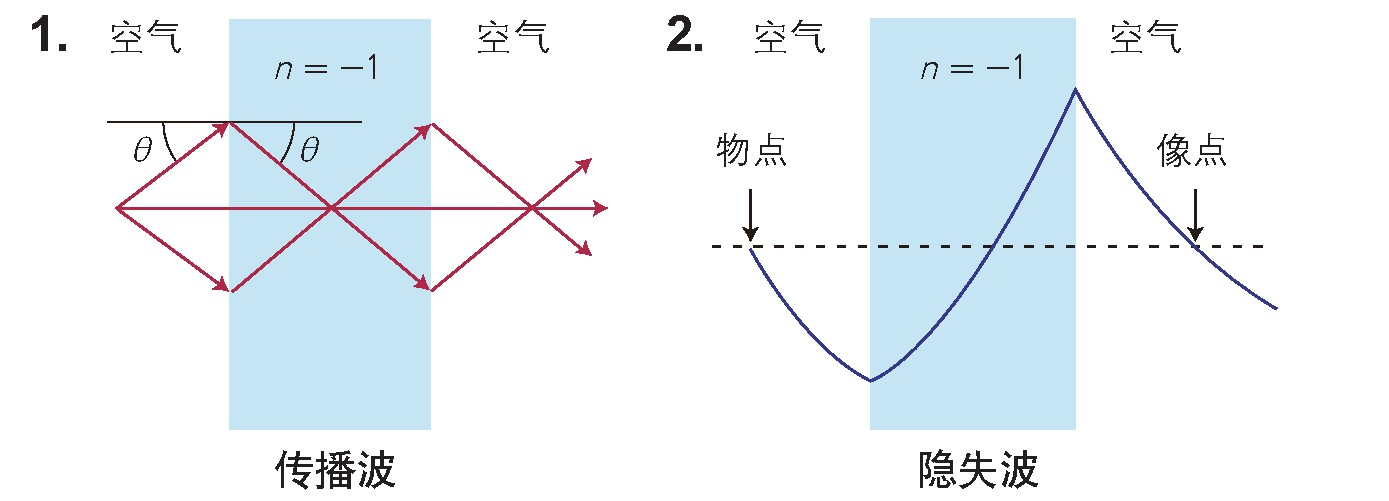
\includegraphics{perfect_lens.jpg}
\caption{完美透镜的原理}   
\end{figure}


早在2005年,研究人员就制造出了分辨率为60nm的超材料透镜(在365nm可见光波长下成像),后来又研究出了远场超透镜和双曲超透镜, 
初步解决了原先的透镜在较远距离上无法成像的问题,使得完美透镜这一设想离真正的大规模应用又迈进了一大步。

\begin{figure}[H]
\centering
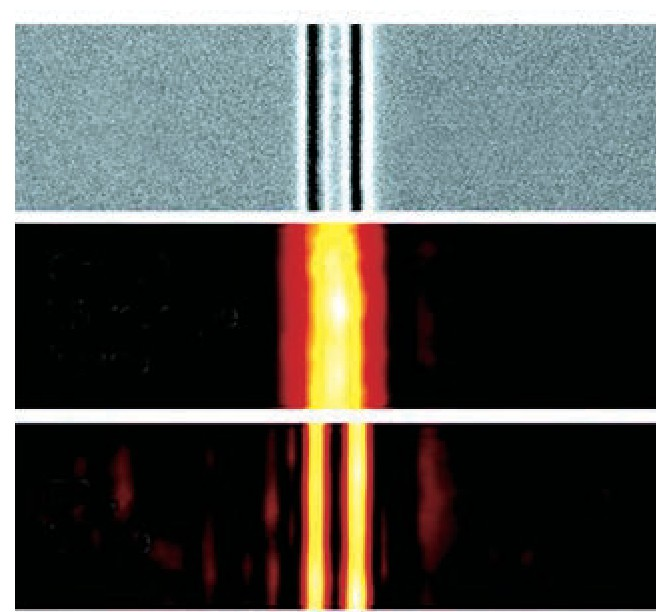
\includegraphics{KXSJ201906013_04800.jpg}
\caption{远场超透镜成像的实例:上图为扫描电子显微镜下观察到的一对宽度为50nm、间隔为70nm的线条;中图为在377纳米的可见光下
用常规透镜对该物体观察时, 两条线不能被分开;下图为超透镜在同样光线下对同一物体观察的结果, 两条线能够被清晰地分开}  
\end{figure}

\subsubsection{隐身技术}
谈到超材料,一个最为魔幻的应用当然要属“隐身”技术,我们常常说的隐身飞机的“隐身”其实不能算作真正意义上的隐身,隐身飞机往往
是通过吸收电磁波或者将电磁波反射到别处来防止被雷达检测到。超材料实现的隐身是指我们可以人为的制造一种材料使得电磁波(光)能够绕开物体继续传播,那么
由于光线没有被吸收,也没有经过物体被反射,所以我们完全不会感觉到这个物体的存在,也就实现了“隐身”的效果。这一设想在理论上也被Pendry预言
了\cite{RN20}。
\begin{figure}[htbp]
\centering
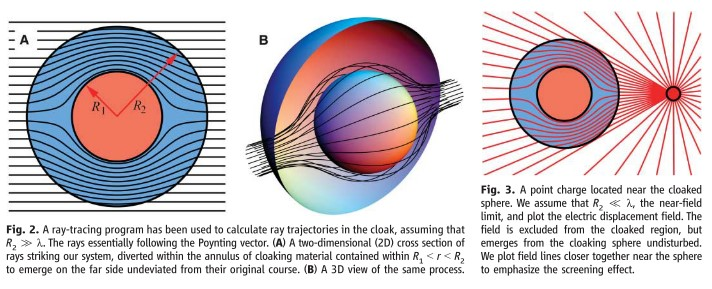
\includegraphics[width=\textwidth]{wave.jpg}
\caption{人为操纵电磁波}   
\end{figure}


也就是说要实现隐身,我们就要通过扭曲物体周围的光线来达成目的,扭曲光线这一点其实并不新鲜,我们通常所知道的海市蜃楼
就是利用了大气受热不均匀导致不同高度处的折射率不同而弯曲光线,但人的视觉总是认为光是沿直线传播的,这也就造成了沙漠绿洲
的假象。有了超材料,折射率可以为负值,那么我们就更容易去按照我们的想法去扭曲光线,依照的基本原理就是麦克斯韦方程组和
其他数学工具,或者说\textbf{变换光学(Transformation Optics)},来构造出一种折射率分布,再来设计材料,就可以实现隐身斗篷了。当然这种隐身也有一个致命缺点,虽然对外面的
人来说,里面的物体隐身了,但是里面的物体同时也无法看见外界,所以还需要进行改进。在探索隐身技术的过程中,曾经在完美透镜
的制作中有着卓业贡献的张翔教授课题组再次崭露头角,率先在2015年做出了一个轻薄且富有柔性的的超材料, 能够覆盖在任意形状的物体上实现隐身效果。
隐身技术或许能在不久后走向实用。

\subsubsection{幻觉}
和隐形技术极为相似,我们或许也能通过弯曲光线来达到另一种效果。比如有两个物体A,B,我们已知光线在物体A附近的光路,我们也就可以
尝试改造物体B附近的光路,使其与物体A相同,这样物体B看起来就会和A一模一样,也就是说我们实现了一种幻像。

\section{其它超材料}
虽说光学超材料是超材料研究的发端和热门领域, 但近些年来, 超材料的概念已经全面扩展到其他领域。例如力学超材料在泡沫
等现有多孔材料的基础上, 通过进一步优化材料内部的网络结构, 不仅可以得到机械性能更加优异的轻质材料, 还能实现独特的力学性质。
譬如当固体在某个方向上被拉伸时, 常规的固体材料由于体积的不可压缩性, 在另外两个方向会收缩, 而某些力学超材料却可以在这两个方向上
发生膨胀。又如热学超材料借鉴光学超材料中的概念, 能够实现与光隐身相似的“热隐身”。还有声学超材料, 能像光学超材料操控电磁波
那样操控声波(将物体的等效质量和等效弹性模量都变为负数), 同样实现了负折射、声波聚焦、声波完美吸收器、声波隐身等功能。


最近比较热门的是一种可以辐射制冷的材料,它能够将射入的大部分电磁波,同时又类似黑体辐射一般辐射出电磁波,起到了降温的效果。
随着人工智能,无人驾驶技术的兴起,在无人驾驶中往往涉及到大量的图像需要即时处理,这个时候如果经过计算机会造成较大的延迟,计算机
处理图像时提取到的是图像的边缘信息,是在对图像进行微分操作。我们其实也可以制造出一种光学超材料来使用光对图像直接进行微分,
不用再到计算机上进行处理,或者减少了计算机的处理量,这样也就相对减少了延迟,在未来需要极低延迟的领域有着很大的应用。
\begin{figure}[htbp]
\centering
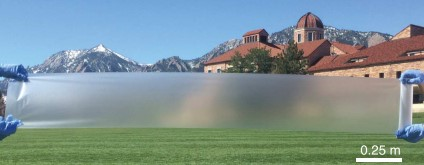
\includegraphics[width=\textwidth]{cooling.jpg}
\caption{一种辐射制冷材料\cite{RN14}}   
\end{figure}


仍有许多超材料还停留在理论层面,比如Stanene,它是一种拓扑绝缘体,由一个原子厚的锡片组成,与石墨烯类似,所以又称锡烯,是一种在过去十年中一直吸引着研究人员的新型材料。虽然这
种材料的内部是电绝缘体,但外部边缘和表面是导电的。如果利用得当,拓扑绝缘体的这种奇怪特性可以使电子无阻力地流动。也就是说
它可能称为科学家们一直在寻找的室温超导体。一旦走出理论用于实践,将会在我们的电子产品和能源消耗方面产生革命性的影响。


\section{结语}
超材料的研究历史很久远,但是实践上依旧是个难题,目前超材料在应用方面还有很长的一段路要走。在超材料方向上的研究,是人类对
大自然的一种挑战,人类并未违背大自然的法则,只是使用这一法则创建了一些看似具有不可能的性质的材料,每种材料具有的每一种超
常性质都会给人类的生活带来翻天覆地的变化。这在某种程度上也是大自然在向人类展现其不可思议的一面。


超材料的理论进展一直比较迅速,科研人员总是能想到一些精妙的点子,但是实践上却因为制造精度等原因,许多超材料只能停留在理论阶段。
近年来, 光刻、3D打印等加工技术的发展使得科学家们在构建复杂结构时越来越得心应手。相信在不远的将来我们将会感受到超材料给我们的生活带来的
便利。

\bibliographystyle{unsrt}
\bibliography{refer}
\end{document}